%%%%%%%%%%%%%%%%%%%%%%%%%%%%%%%%%%%%%%%%%%%%%%%%%%%%%%%%%%%%%%%%%%%%%%%%%%%%%%%
%%% SETUP

\providecommand{\main}{../..}  % for subfiles
\providecommand{\mystyleloc}{../../util}  % for stylesheets
\documentclass[\main/main.tex]{subfiles}

%%%%%%%%%%%%%%%%%%%%%%%%%%%%%%%%%%%%%%%%%%%%%%%%%%%%%%%%%%%%%%%%%%%%%%%%%%%%%%%
%                                 SETTINGS
%%%%%%%%%%%%%%%%%%%%%%%%%%%%%%%%%%%%%%%%%%%%%%%%%%%%%%%%%%%%%%%%%%%%%%%%%%%%%%%
% Implementing Package Settings

\graphicspath{{images/}{\main/images/}}

\title{General Qualifying Exam Solutions: Cosmology\\}
\author{{Starkman}, Nathaniel \\%
		\and {Lokken}, Martine \\%
		\and {Ludwig}, Bethany \\%
		\and {Winch}, Harrison \\%
		\and {Sheere}, Connor \\%
		\and {Sheere}, Connor%
}
% \date{\today}


%%%%%%%%%%%%%%%%%%%%%%%%%%%%%%%%%%%%%%%%%%%%%%%%%%%%%%%%%%%%%%%%%%%%%%%%%%%%%%%
%                                  DOCUMENT
%%%%%%%%%%%%%%%%%%%%%%%%%%%%%%%%%%%%%%%%%%%%%%%%%%%%%%%%%%%%%%%%%%%%%%%%%%%%%%%

\begin{document}

% -----------------------------------------------------------------------------
%                                  TITLE PAGE
% -----------------------------------------------------------------------------

\maketitle

% -----------------------------------------------------------------------------
%                                     TOC
% -----------------------------------------------------------------------------

\tableofcontents
\let\tableofcontents\relax


% -----------------------------------------------------------------------------
%                                    INTRO
% -----------------------------------------------------------------------------

\newpage
\section{Introduction} % (fold)
\label{sec:introduction}


	% External Answers
	\includepdf[pagecommand=\subsection{Campbell Cosmo Intro},scale=.95,pages=2,]{cosmo_extragal/Campbell/cosmology}\includepdf[pagecommand=\large{Campbell Cosmo Intro},scale=.95,pages=3-5,]{cosmo_extragal/Campbell/cosmology}

	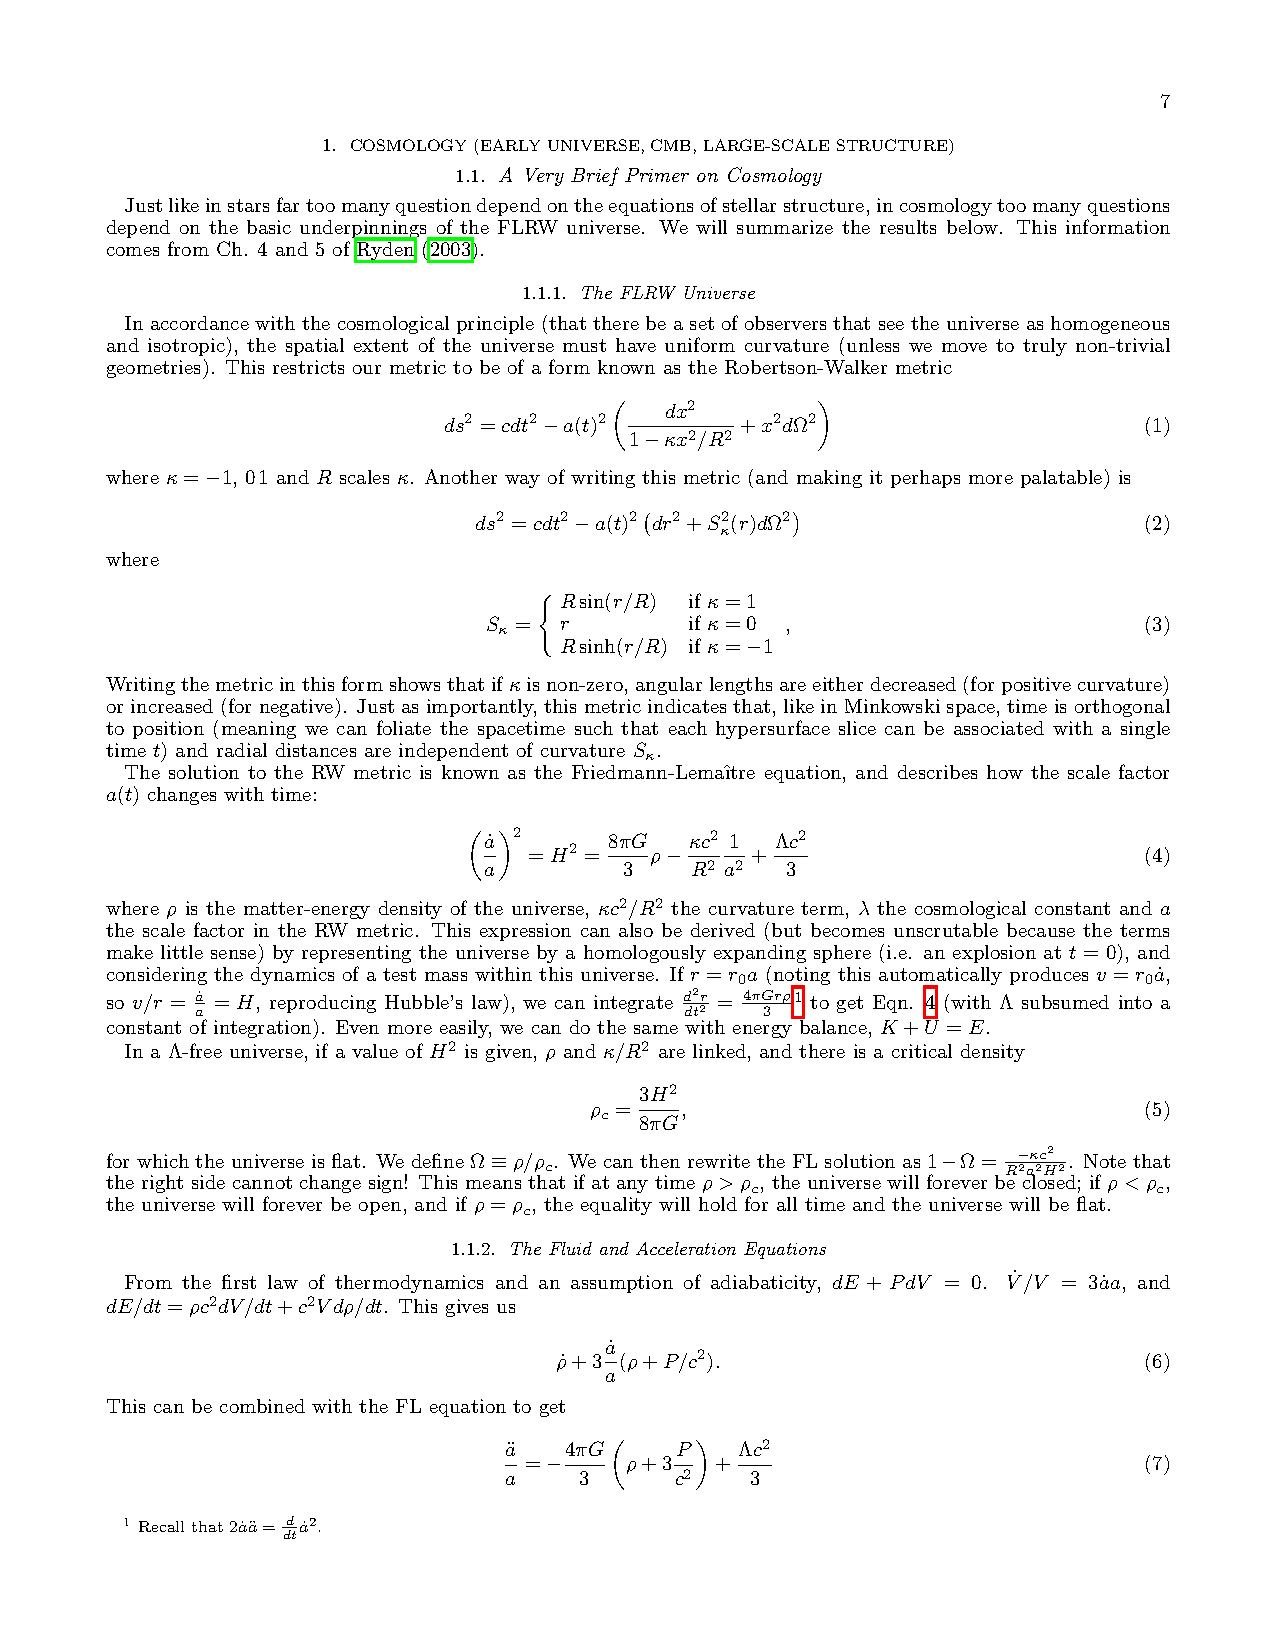
\includepdf[pagecommand=\subsection{Zhu Intro},pages=1]{cosmo_extragal/Zhu/Zhu_Intro}\includepdf[pagecommand=\large{Zhu Intro},pages=2-]{cosmo_extragal/Zhu/Zhu_Intro}

% section introduction (end)

% -----------------------------------------------------------------------------
%                                      Q1
% -----------------------------------------------------------------------------

\section{Q1) Recombination} % (fold)
\label{sec:q1_recombination}
\questiontext{What is recombination? At what temperature did it occur? Explain why this does not match the ionization potential of hydrogen.}

	\subsection{Short Answer} % (fold)
	\label{sub:short_answer}
	{\it (From Campbell Answers)}

		Recombination refers to the time at which the temperature of the early Universe became cool enough such that it was thermodynamically favorable for the ionized plasma of free electrons and ions to couple and form neutral atoms. Numerically, this might be defined as the moment when the number density of ions is equal to the number density of neutral atoms.\\

		Temperature: ${\mathbf T \sim 1,000\,{\rm K}}$ (corresponding to an energy of $\sim 0.1\,{\rm eV}$) at a redshift of $z \sim 1,100$.\\

		This does not match the ionization potential of hydrogen because the early Universe (as it was hot and dense) can be described by a blackbody with a characteristic distribution of photon energies including an exponential tail of high energy photons (Wein's tail). While the peak of the blackbody spectrum describing the temperature of the early Universe is below the ionization energy of hydrogen, the photons in the high-energy exponential tail of the blackbody spectrum have sufficient energies for photoionization.

	% subsection short_answer (end)

	\subsection{Cosmology Class Fall 2019: Martine's Notes} % (fold)
	\label{sub:cosmology_class_fall_2019_martine_s_notes}

		Steps: Integrate blackbody to find what percentage of photons have energies higher than 13.6 eV.
	    Extrapolate measured $\Omega_b$ back in time to get the photon to baryon ratio.
	    The number of photons above 13.6 eV equals number of baryons at 5600 K. 
	    
	    \begin{equation}
	        X_p = \frac{N_p}{N_p + N_H} \approx 0.1
	    \end{equation}
	    at $T_{rec}$.
	    
	    Saha equation:
	    \begin{equation}
	        \frac{X^2}{1-X} = \frac{(2\pi m_e kT)^{3/2}}{(n_e + n_H)(2\pi h)^3} e^{-13.6eV/kT}
	    \end{equation}
	    At what temperature is $X$ 10\%?
	    Depends on $\Omega_b h^2$ because of the $(n_e + n_H)$ in denominator. Higher density of baryons makes recombination happen earlier. Solving for when $X_p$ is 0.1 gives $T\sim 3600K$ or 0.3 eV. This is recombination.
	    
	    Then ask, when will the universe be 'transparent'? Can define that by when optical depth $\tau = 1$. This comes out to be $T\sim3200$K, $z\sim1100$. This is decoupling.
	    
	    \textbf{Barth's Follow Up Questions}
	     Approximately how long did the process of recombination take (define however is convenient)?
	
	% subsection cosmology_class_fall_2019_martine_s_notes (end)


	% External Answers
	\includepdf[pagecommand=\subsection{Q1) Ludwig Cosmo Q1},pages=3]{cosmo_extragal/Ludwig/Cosmology}

	\includepdf[pagecommand=\subsection{Q1) Herman Cosmo Q1},scale=.93, offset=0 -14,pages=1]{cosmo_extragal/Herman/1_Cosmology}

	\includepdf[pagecommand=\subsection{Q1) Campbell Cosmo Q1},scale=.95,pages=6]{cosmo_extragal/Campbell/cosmology}\includepdf[pagecommand=\large{Q1) Campbell Cosmo Q1},scale=.95,pages=7]{cosmo_extragal/Campbell/cosmology}

	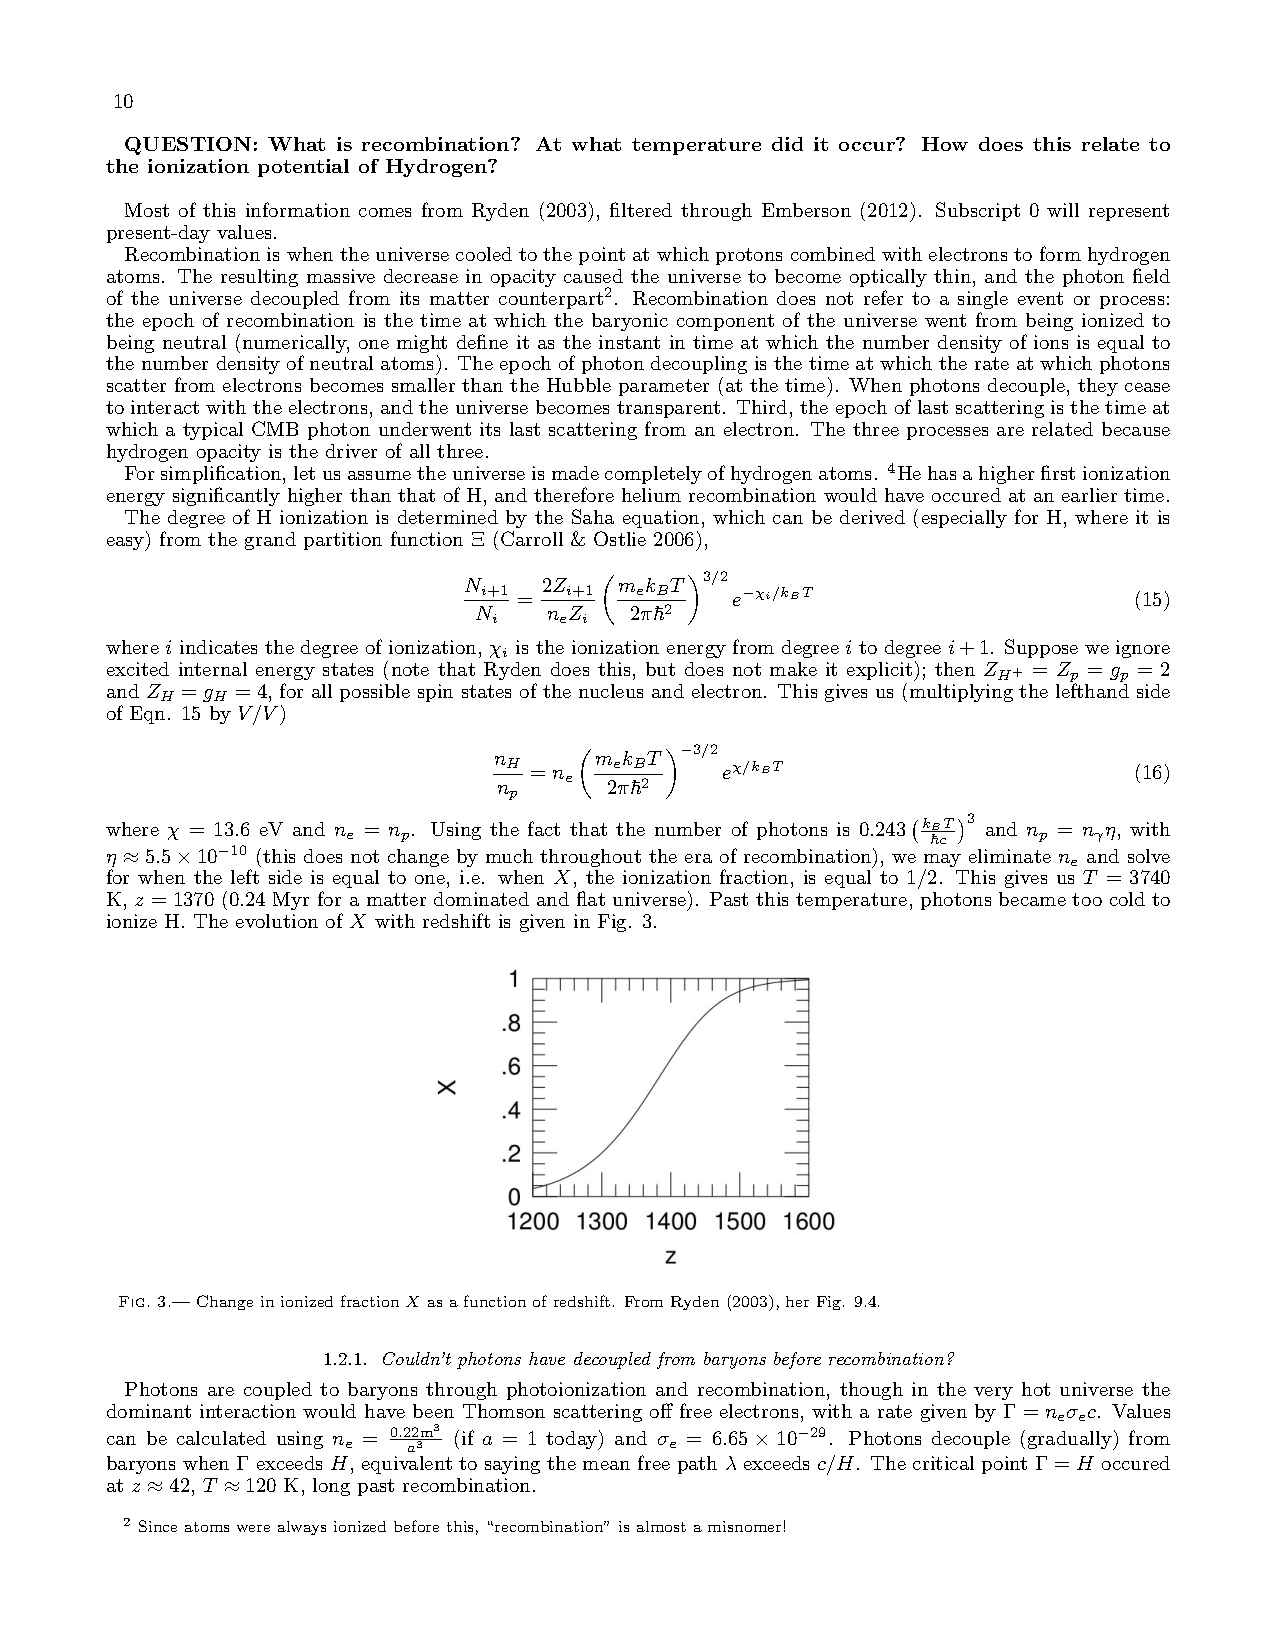
\includepdf[pagecommand=\subsection{Q1) Zhu Cosmo Q1},pages=1]{cosmo_extragal/Zhu/Zhu_Q1}\includepdf[pagecommand=\large{Zhu Cosmo Q1},pages=2-]{cosmo_extragal/Zhu/Zhu_Q1}

% section q1_recombination (end)


% -----------------------------------------------------------------------------
%                                      Q2
% -----------------------------------------------------------------------------
\newpage
\section{Q2) Flat Universe Properties} % (fold)
\label{sec:q2_flat_universe_properties}
\questiontext{The universe is said to be “flat”, or, close to flat. What are the properties of a flat universe and what evidence do we have for it?}

	\subsection{Short Answer} % (fold)
	\label{sub:short_answer}

	The three properties of a flat universe are:

	\begin{enumerate}
		\item parallel lines never converge or diverge
		\item angles in a triangle sum to 180 degrees
		\item the universe is at the critical density
	\end{enumerate}

	The first two are geometric properties of a flat space. The third is a statement of the universe's energy content.

	The Friedmann Equation is  ${H(t)}^2 = \frac{8 \pi G}{3} \left[ \rho(t) + \frac{\rho_{crit} -\rho_0}{{a(t)}^2} \right], \rho_k \equiv \rho_{crit} -\rho_0$.

	Therefore, $\rho_k = 0 \rightarrow \rho_0 = \rho_{crit}$

	There is a lot of evidence for a flat universe

	\begin{enumerate}
		\item direct measurements of the universe's density: CMB power spectrum, galaxy cluster distribution.
		\item Angular scale of CMB peak: positive curvature moves peak to larger angular scales (lower $l$). Vice versa for negative curvature.
		\item map the expansion rate with Type Ia SNR.
	\end{enumerate}	
	
	% subsection short_answer (end)


	% External Answers
	\includepdf[pagecommand=\subsection{Q2) Ludwig Cosmo Q2},pages=4]{cosmo_extragal/Ludwig/Cosmology}

	\includepdf[pagecommand=\subsection{Q2) Herman Cosmo Q2},scale=.93, offset=0 -14,pages=2]{cosmo_extragal/Herman/1_Cosmology}\includepdf[pages=8,pagecommand=\subsection{Q2) Campbell Cosmo Q2},scale=.95]{cosmo_extragal/Campbell/cosmology}\includepdf[pages=9-10,pagecommand=\large{Campbell Cosmo Q2},scale=.95]{cosmo_extragal/Campbell/cosmology}

	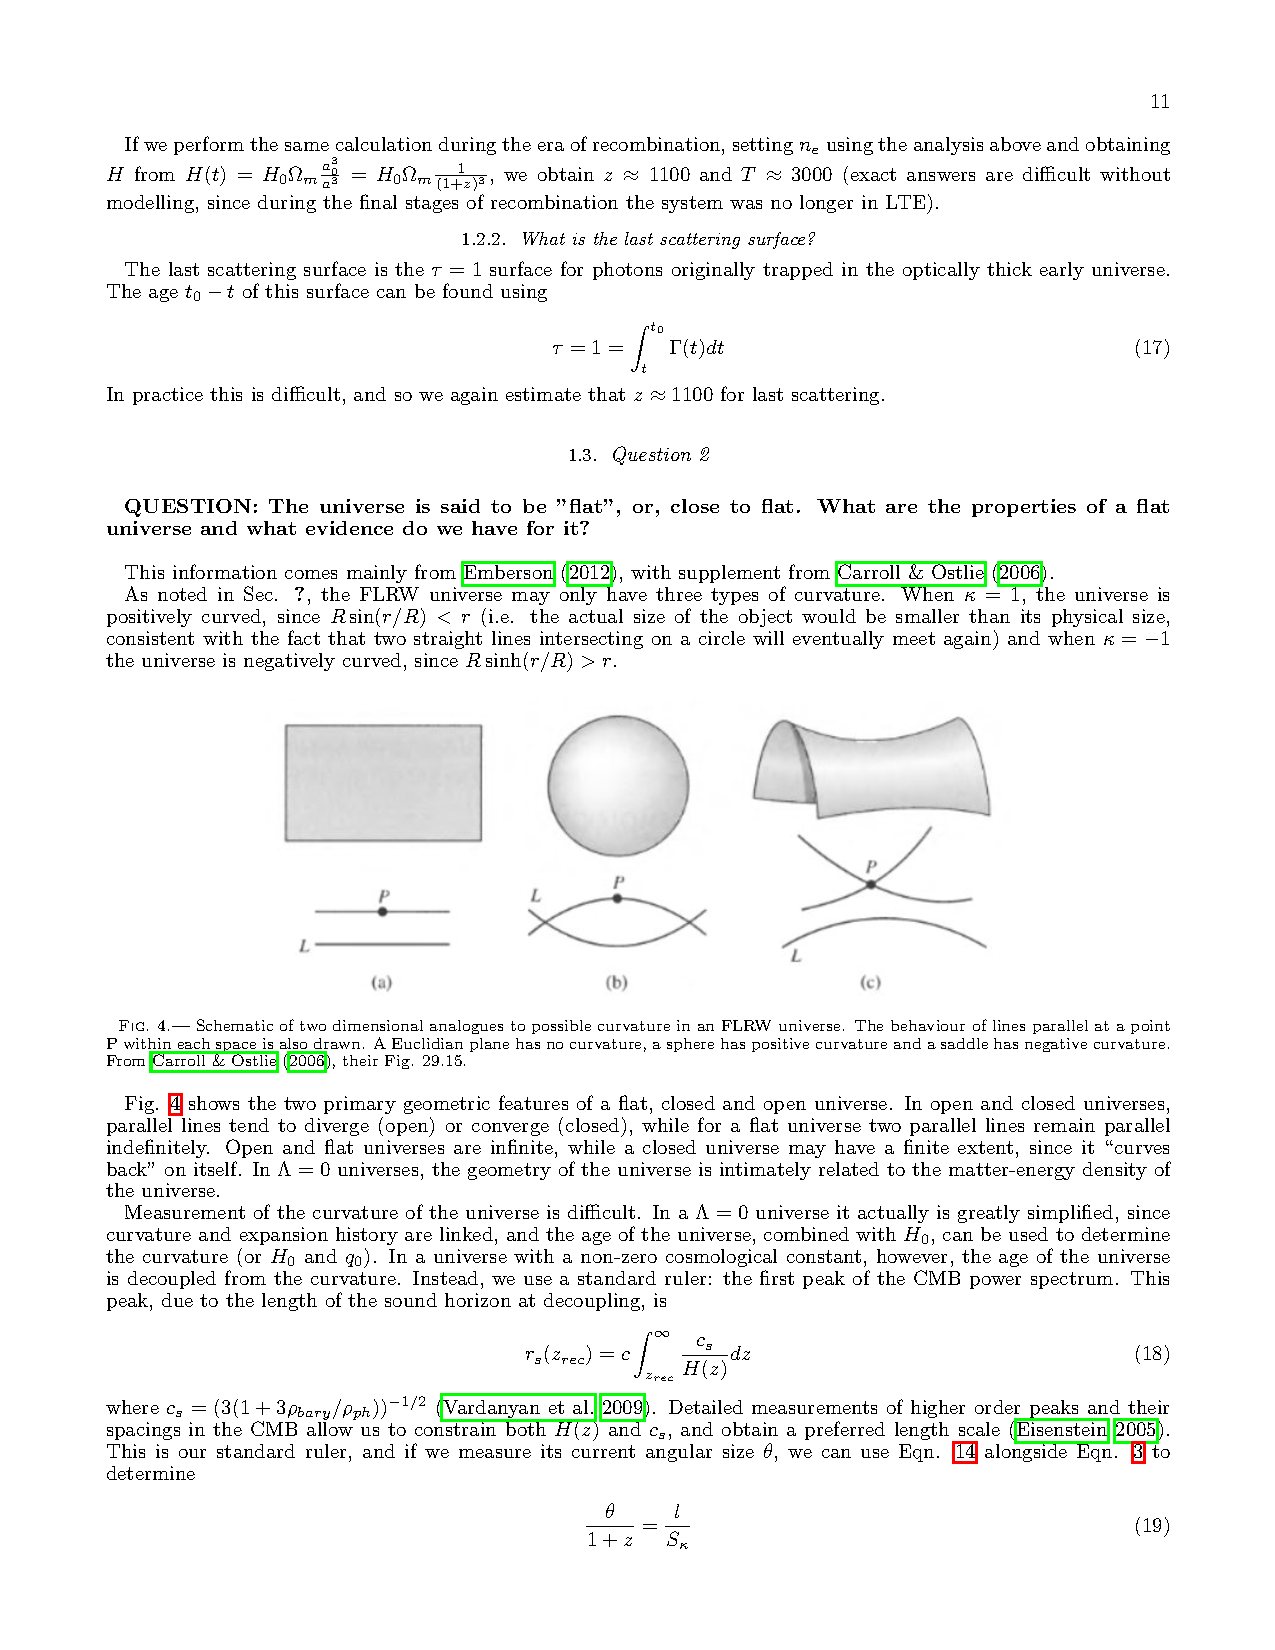
\includepdf[pagecommand=\subsection{Q2) Zhu Cosmo Q2},pages=1]{cosmo_extragal/Zhu/Zhu_Q2}\includepdf[pages=2-]{cosmo_extragal/Zhu/Zhu_Q2}

% section q2_flat_universe_properties (end)

% -----------------------------------------------------------------------------
%                                      Q3
% -----------------------------------------------------------------------------

\newpage
\section{Q3) Term Definitions} % (fold)
\label{sec:q3_term_definitions}
\questiontext{Define and describe the following terms: Comoving Distance, Proper Distance, Angular Diameter Distance, Luminosity Distance, Proper Time, Coordinate Time}

	\subsection{Short Answer} % (fold)
	\label{sub:short_answer}


	$E(Z) = \sqrt{\Omega_r a^{-4} + \Omega_m a^{-3} + \Omega_k a^{-2} + \Omega_\Lambda}$

	$d_H = c / H_0$

	{\it Comoving Distance}: ``the distance between two points measured along a path defined at the present cosmological time. For objects moving with the Hubble flow, it is deemed to remain constant in time.'' (\href{https://en.wikipedia.org/wiki/Comoving_and_proper_distances}{Wikipedia})

		$\chi = \int_{t_e}^{t} c \frac{\dif{t'}}{a(t')} = d_H \int_{0}^{z} c \frac{\dif{z'}}{E(z')}$

	$  \chi = \left\{
	\begin{array}{ll}
	      |\kappa|^{-1/2} \inv{\sinh}{\sqrt{|\kappa|r}} & \kappa<0 (negatively curved, hyperbolic universe) \\
	      r & \kappa=0 (flat universe) \\
	      |\kappa|^{-1/2} \inv{\sin}{\sqrt{|\kappa|r}} & \kappa>0 (positively curved, spherical universe) \\
	\end{array} 
	\right. $

	Solving for $r \equiv d_M$, the {\it transverse comoving distance}.


	{\it Transverse Comoving Distance}:

	$  d_M = \left\{
	\begin{array}{ll}
	      \frac{d_H}{\sqrt{\Omega_k}} \sinh\left(\sqrt{\Omega_k} d_C(z) / d_H\right) & \Omega_k > 0 (negatively curved, hyperbolic universe) \\
	      d_C(z) & \kappa=0 (flat universe) \\
	      \frac{d_H}{\sqrt{|\Omega_k}|} \sin\left(\sqrt{|\Omega_k|} d_C(z) / d_H\right) & \Omega_k > 0 (positively curved, spherical universe) \\
	\end{array} 
	\right. $


	{\it Proper Distance}: $d_p(t) = a(t) \chi$. The proper distance between two points at time $t$ is just the distance that would be measured by rulers between them at that time.


	{\it Angular Diameter Distance}: $d_A = a(t) d_M$

	{\it Luminosity Distance}: $d_L = d_M / a(t)$

	{\it Light travel Distance}: $d_T(z) = d_H \int_{0}{z} \frac{\dif{z'}}{(1+z')E(z')}$


	{\it Proper time}: the observer's time

	{\it conformal time}: $\dif{\tau} = \dif{t} / a$


	% External Answers
	

% section q4_big_bang_evidence (end)


% -----------------------------------------------------------------------------
%                                      Q4
% -----------------------------------------------------------------------------

\newpage
\section{Q4) Big Bang Evidence} % (fold)
\label{sec:q4_big_bang_evidence}
\questiontext{State and explain three key pieces of evidence for a Big Bang origin for the observable Universe.}

	\subsection{Short Answer} % (fold)
	\label{sub:short_answer}
	{\it from Campbell's Notes}
	
	The success of the Big Bang (BB) rests on three observational pillars:

	\begin{enumerate}
	    \item Hubble's Law exhibiting expansion: If the Universe is expanding at the present time, then by `turning back the clock' the Universe must have been much smaller in the past. Hence, the BB.
	    \item Light element abundances which are in accord with Big Bang nucleosynthesis: When the Universe was still a very hot plasma, the extreme radiation field ensured that any nucleus produced would be immediately photoionized by a high energy photon. As the Universe cooled (via expansion) well below the typical binding energies of nuclei, light elements began to form. Knowing the conditions of the early Universe and the relevant cross sections, one can calculate the expected primordial abundances of these light elements. Such predictions are consistent with measurements.
	    \item The blackbody radiation left over from the first few hundred thousand years, the cosmic microwave background: The fact that the early Universe was very hot and dense meant that the baryonic matter was well coupled with the radiation field implying thermal equilibrium (TE) of photons. In TE, photons should follow the blackbody (or Planck) function in which the energy density is only dependent on temperature. As it turns out, the CMB radiation is the most accurate BB curve yet to be measured!
	\end{enumerate}

	% subsection short_answer (end)

	\subsection{Relevant Equations} % (fold)
	\label{sub:relevant_equations}

	For Hubble, $v = H_0 d$

	for the CMB, $T = T_0 / a = 2.7 K / a \rightarrow \infty $ as $a \rightarrow 0$
	
	% subsection relevant_equations (end)




	% External Answers
	\includepdf[pagecommand=\subsection{Q4) Ludwig Cosmo Q4},pages=6]{cosmo_extragal/Ludwig/Cosmology}

	\includepdf[pagecommand=\subsection{Q4) Herman Cosmo Q4},scale=.93,offset=0 -14,pages=5]{cosmo_extragal/Herman/1_Cosmology}

	\includepdf[pagecommand=\subsection{Q4) Campbell Cosmo Q4},scale=.93,offset=0 -14,pages=21]{cosmo_extragal/Campbell/cosmology}\includepdf[pagecommand=\large{Q4) Campbell Cosmo Q4},scale=.93,offset=0 -14,pages=22-27]{cosmo_extragal/Campbell/cosmology}

	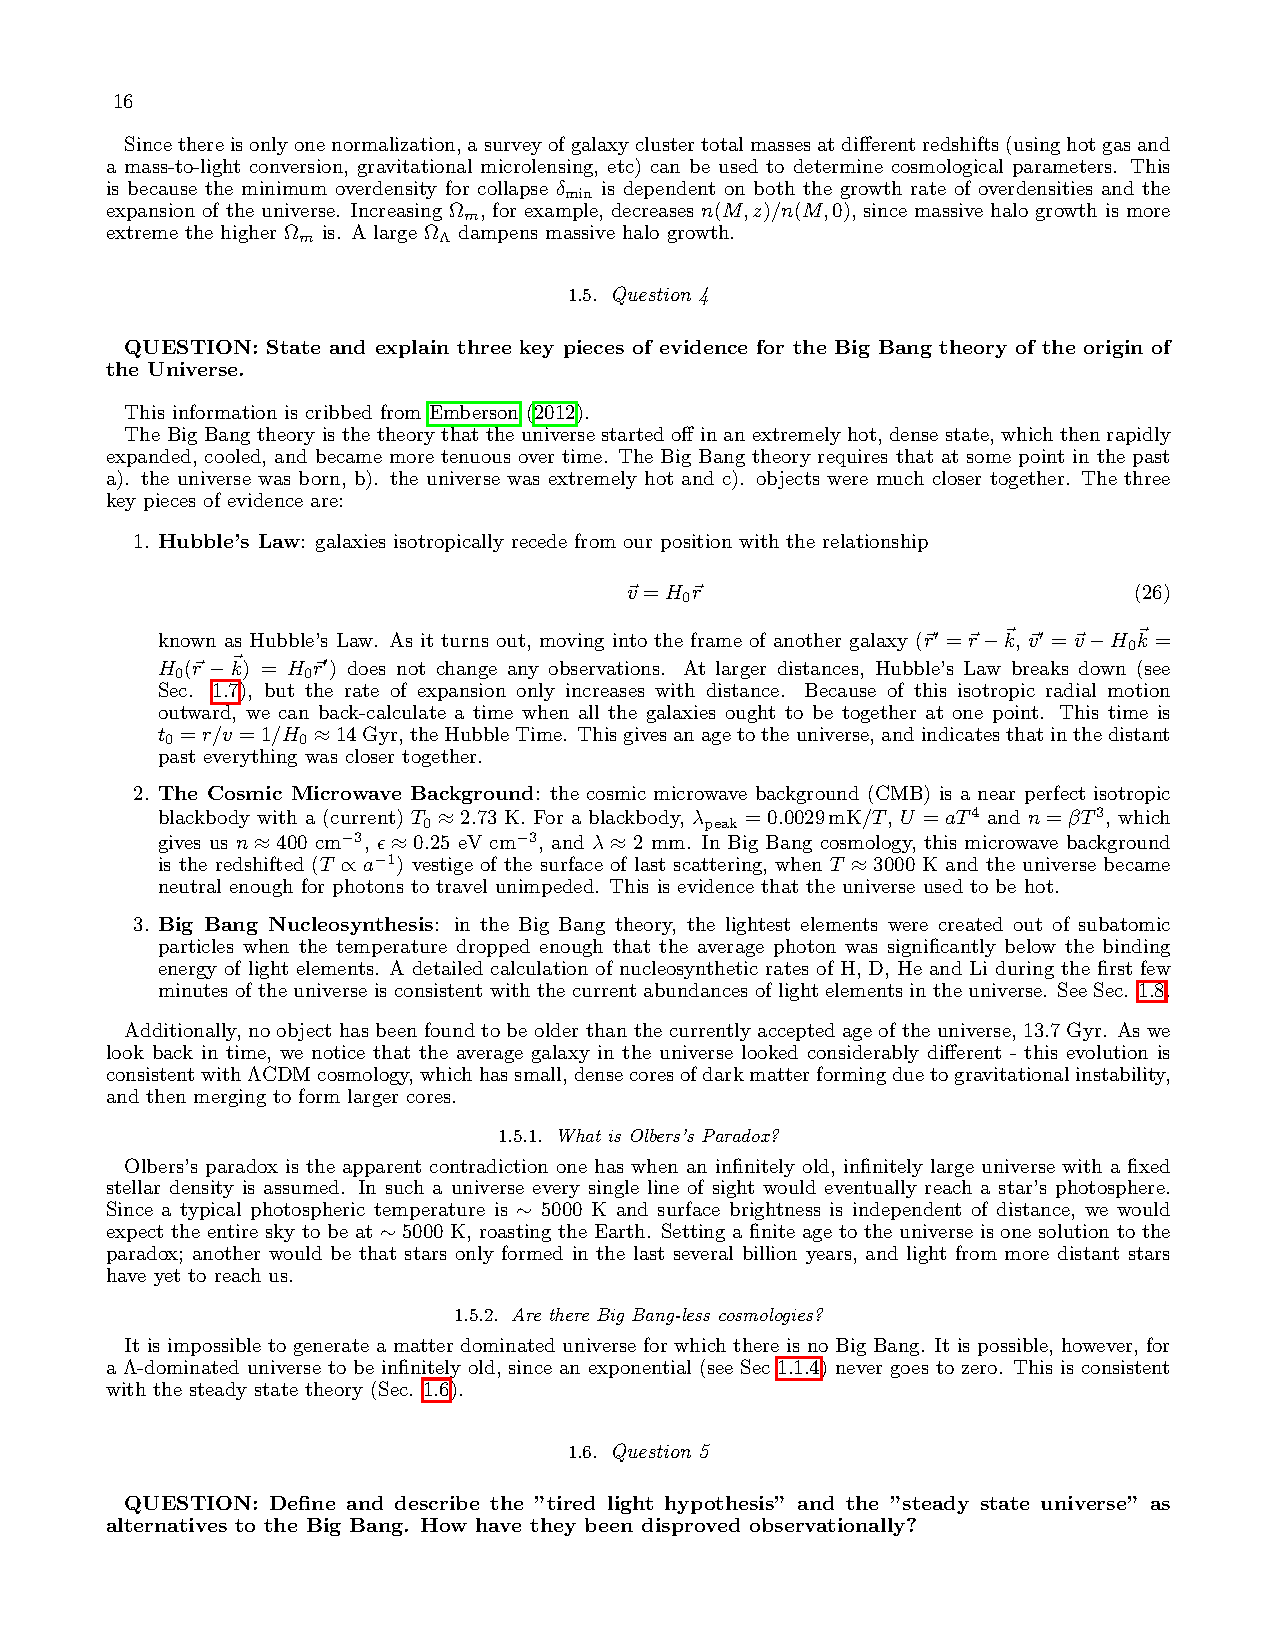
\includepdf[pagecommand=\subsection{Q4) Zhu Cosmo Q4},pages=1]{cosmo_extragal/Zhu/Zhu_Q4}

    \subsection{Cosmology Class Fall 2019: Martine's Notes}

    1. Expansion of the universe. However, this is still possible with the steady-state model where as the universe expands, matter keeps getting created and the same density is maintained. In this model, older galaxies redshift away into nothingness and newer galaxies form into existence from the created matter. The new galaxies look exactly like the old ones so you should see the same distribution of galaxies at any redshift. Observations of quasars at high-redshift (which we don't see at low-redshift) proved that the universe is changing over time so the steady-state model couldn't be true.
    
    The CMB is the best counter to any steady-state model. The universe was clearly very different in the past. It was a hot dense gas. This is only possible if the universe was smaller in the past.
    
    Big bang nucleosynthesis predicts the correct ratio of elements as is measured.
% section q4_big_bang_evidence (end)


% -----------------------------------------------------------------------------
%                                      Q5
% -----------------------------------------------------------------------------

\newpage
\section{Q5) Big Bang Nucleosynthesis (BBN)} % (fold)
\label{sec:q5_big_bang_nucleosynthesis_bbn}
\questiontext{Describe Big Bang nucleosynthesis. Why are only very light elements (H, D, He, and traces of Li) produced?}


	% External Answers
	\includepdf[pagecommand=\subsection{Q5) Ludwig Cosmo Q5},pages=7]{cosmo_extragal/Ludwig/Cosmology}

	\includepdf[pagecommand=\subsection{Q5) Herman Cosmo Q6},scale=.93,offset=0 -14,pages=7]{cosmo_extragal/Herman/1_Cosmology}

	\includepdf[pagecommand=\subsection{Q5) Campbell Cosmo Q6},scale=.93,offset=0 -14,pages=30]{cosmo_extragal/Campbell/Cosmology}\includepdf[pagecommand=\large{Q5) Campbell Cosmo Q6},scale=.93,offset=0 -14,pages=31-32]{cosmo_extragal/Campbell/Cosmology}

	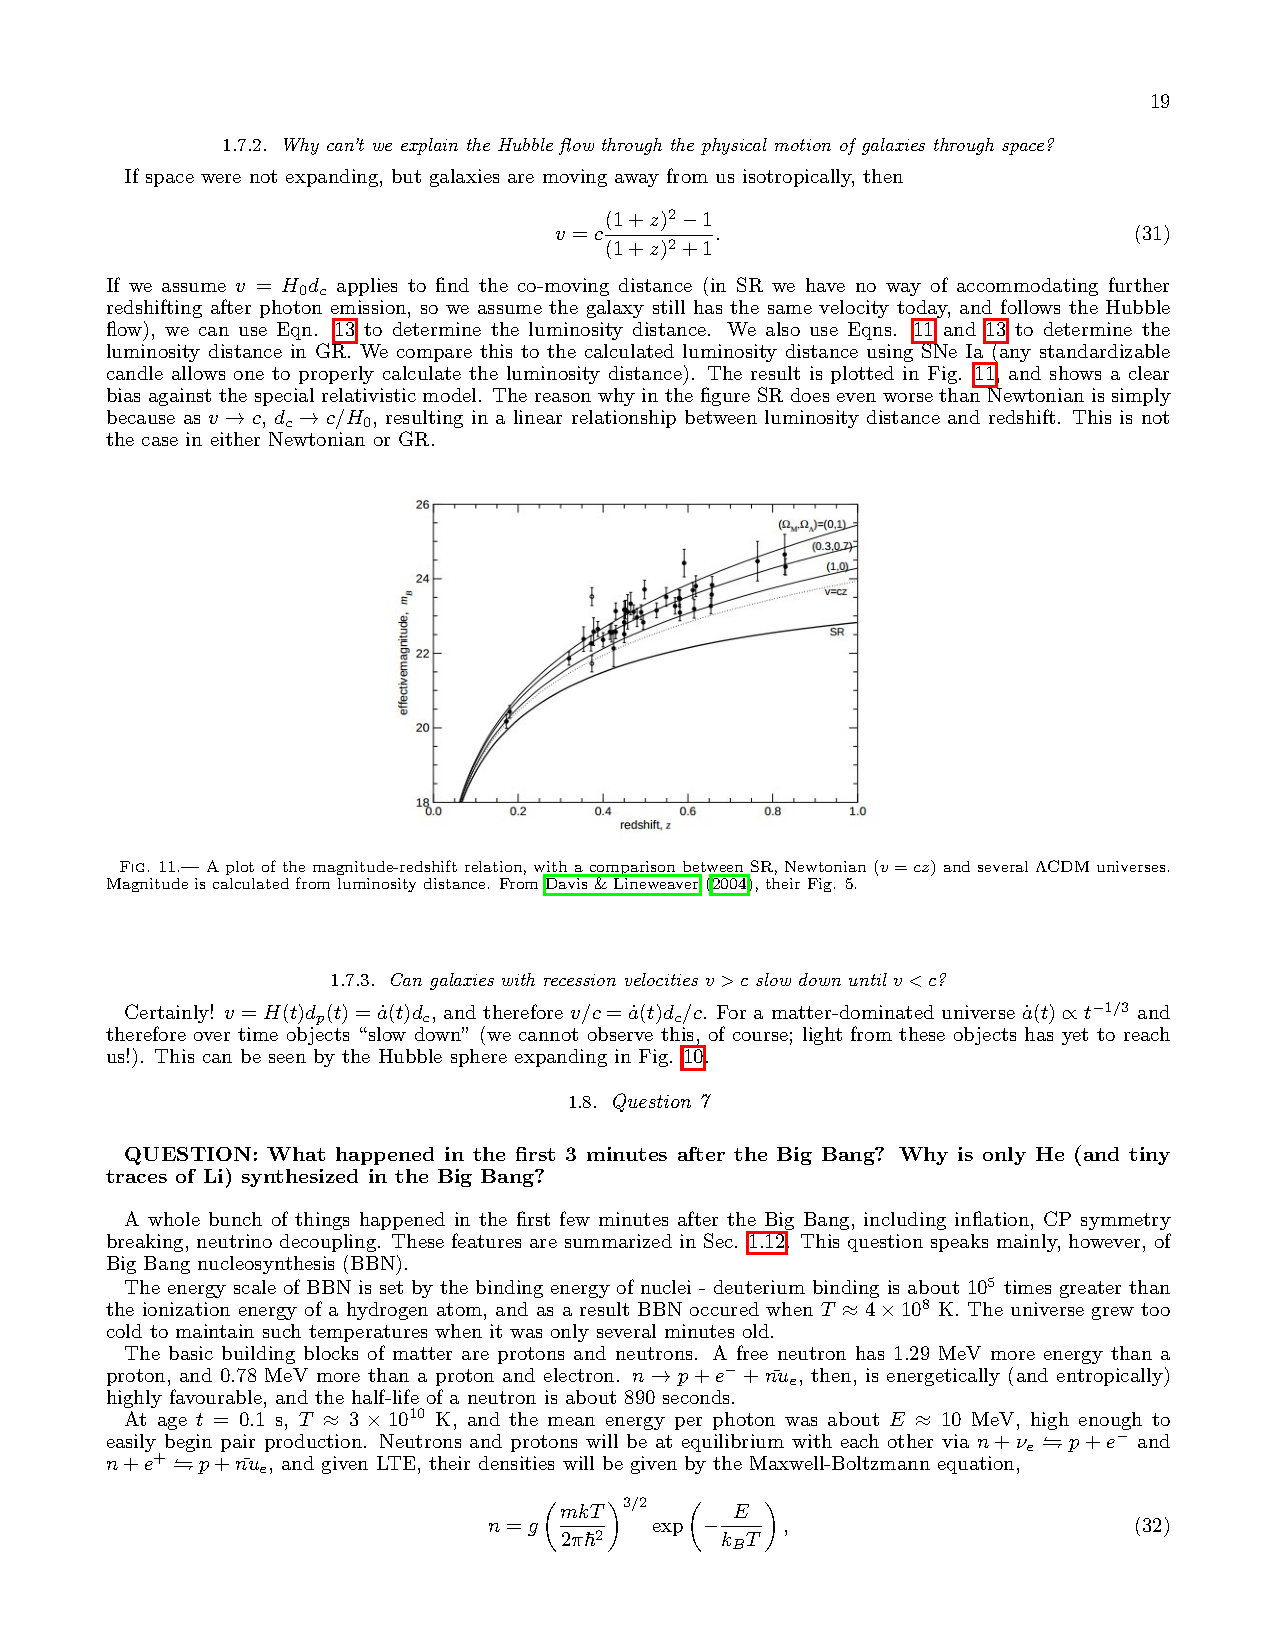
\includepdf[pagecommand=\subsection{Q5) Zhu Cosmo Q5},pages=1]{cosmo_extragal/Zhu/Zhu_Q5_1}\includepdf[pages=2-]{cosmo_extragal/Zhu/Zhu_Q5_1}

% section q5_big_bang_nucleosynthesis_bbn (end)


% -----------------------------------------------------------------------------
%                                      Q6
% -----------------------------------------------------------------------------

\section{Q6) Type 1a Supernovae for Cosmology} % (fold)
\label{sec:q6_type_1a_supernovae_for_cosmology}
\questiontext{Explain how and why Type Ia Supernovae are used in the measurements of cosmological parameters.}


	% External Answers
	\includepdf[pagecommand=\subsection{Q6) Ludwig Cosmo Q6},pages=8]{cosmo_extragal/Ludwig/Cosmology}

	\includepdf[pagecommand=\subsection{Q6) Herman Cosmo Q7},scale=.93,offset=0 -14,pages=8]{cosmo_extragal/Herman/1_Cosmology}

	\includepdf[pagecommand=\subsection{Q6) Campbell Cosmo Q7},scale=.93,offset=0 -14,pages=33]{cosmo_extragal/Campbell/cosmology} \includepdf[pagecommand=\large{Q6) Campbell Cosmo Q7},scale=.93,offset=0 -14,pages=34-39]{cosmo_extragal/Campbell/cosmology}

	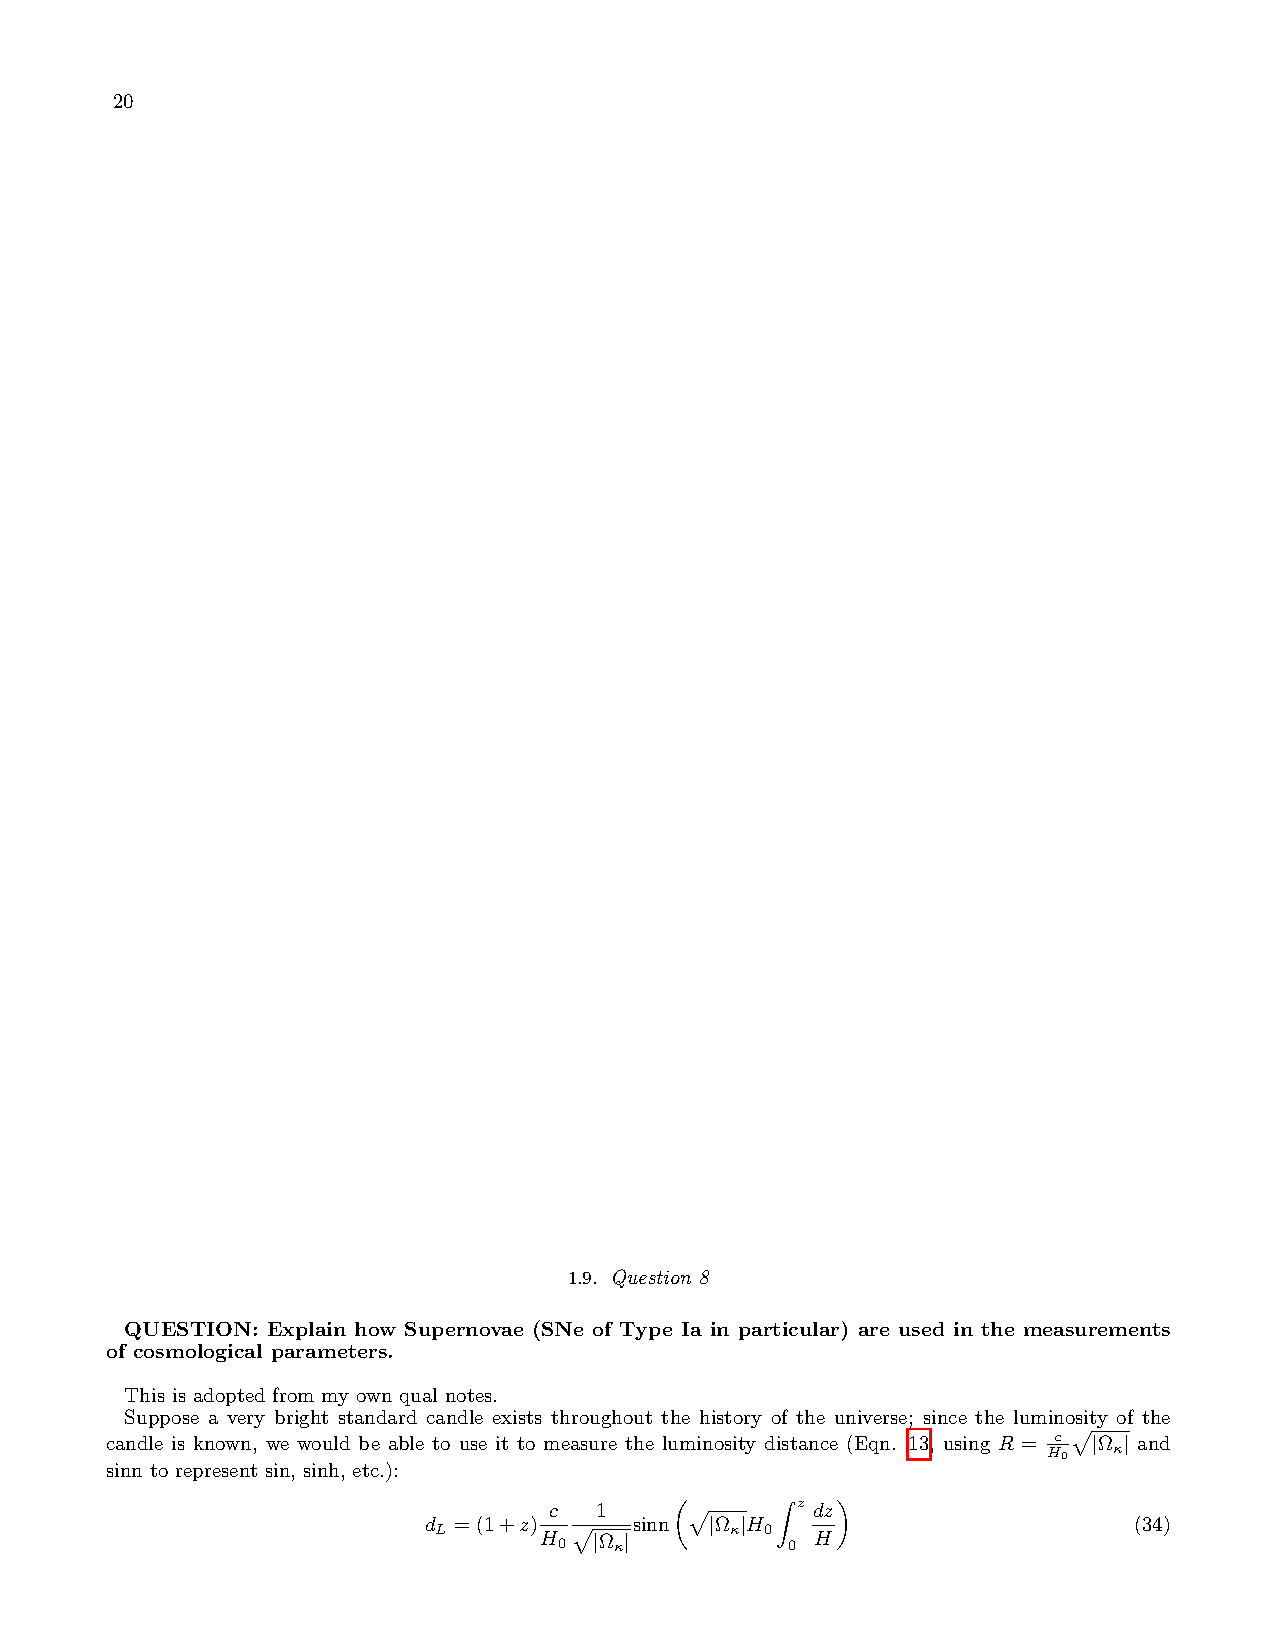
\includepdf[pagecommand=\subsection{Q6) Zhu Cosmo Q8},pages=1]{cosmo_extragal/Zhu/Zhu_Q6}\includepdf[pages=2-]{cosmo_extragal/Zhu/Zhu_Q6}

% section q6_type_1a_supernovae_for_cosmology (end)


% -----------------------------------------------------------------------------
%                                      Q7
% -----------------------------------------------------------------------------

\section{Q7) The distance Ladder} % (fold)
\label{sec:q7_the_distance_ladder}
\questiontext{Describe as many steps of the distance ladder and the involved techniques as you can.}


	% External Answers
	\includepdf[pagecommand=\subsection{Q7) Herman ExtraGal Q3},scale=.93,offset=0 -14,pages=3]{cosmo_extragal/Herman/2_Extragalactic}

	\includepdf[pagecommand=\subsection{Q7) Campbell ExtraGal Q3},scale=.93,offset=0 -14,pages=11]{cosmo_extragal/Campbell/extragalactic}\includepdf[pagecommand=\large{Q7) Campbell ExtraGal Q3},scale=.93,offset=0 -14,pages=12-18]{cosmo_extragal/Campbell/extragalactic}

	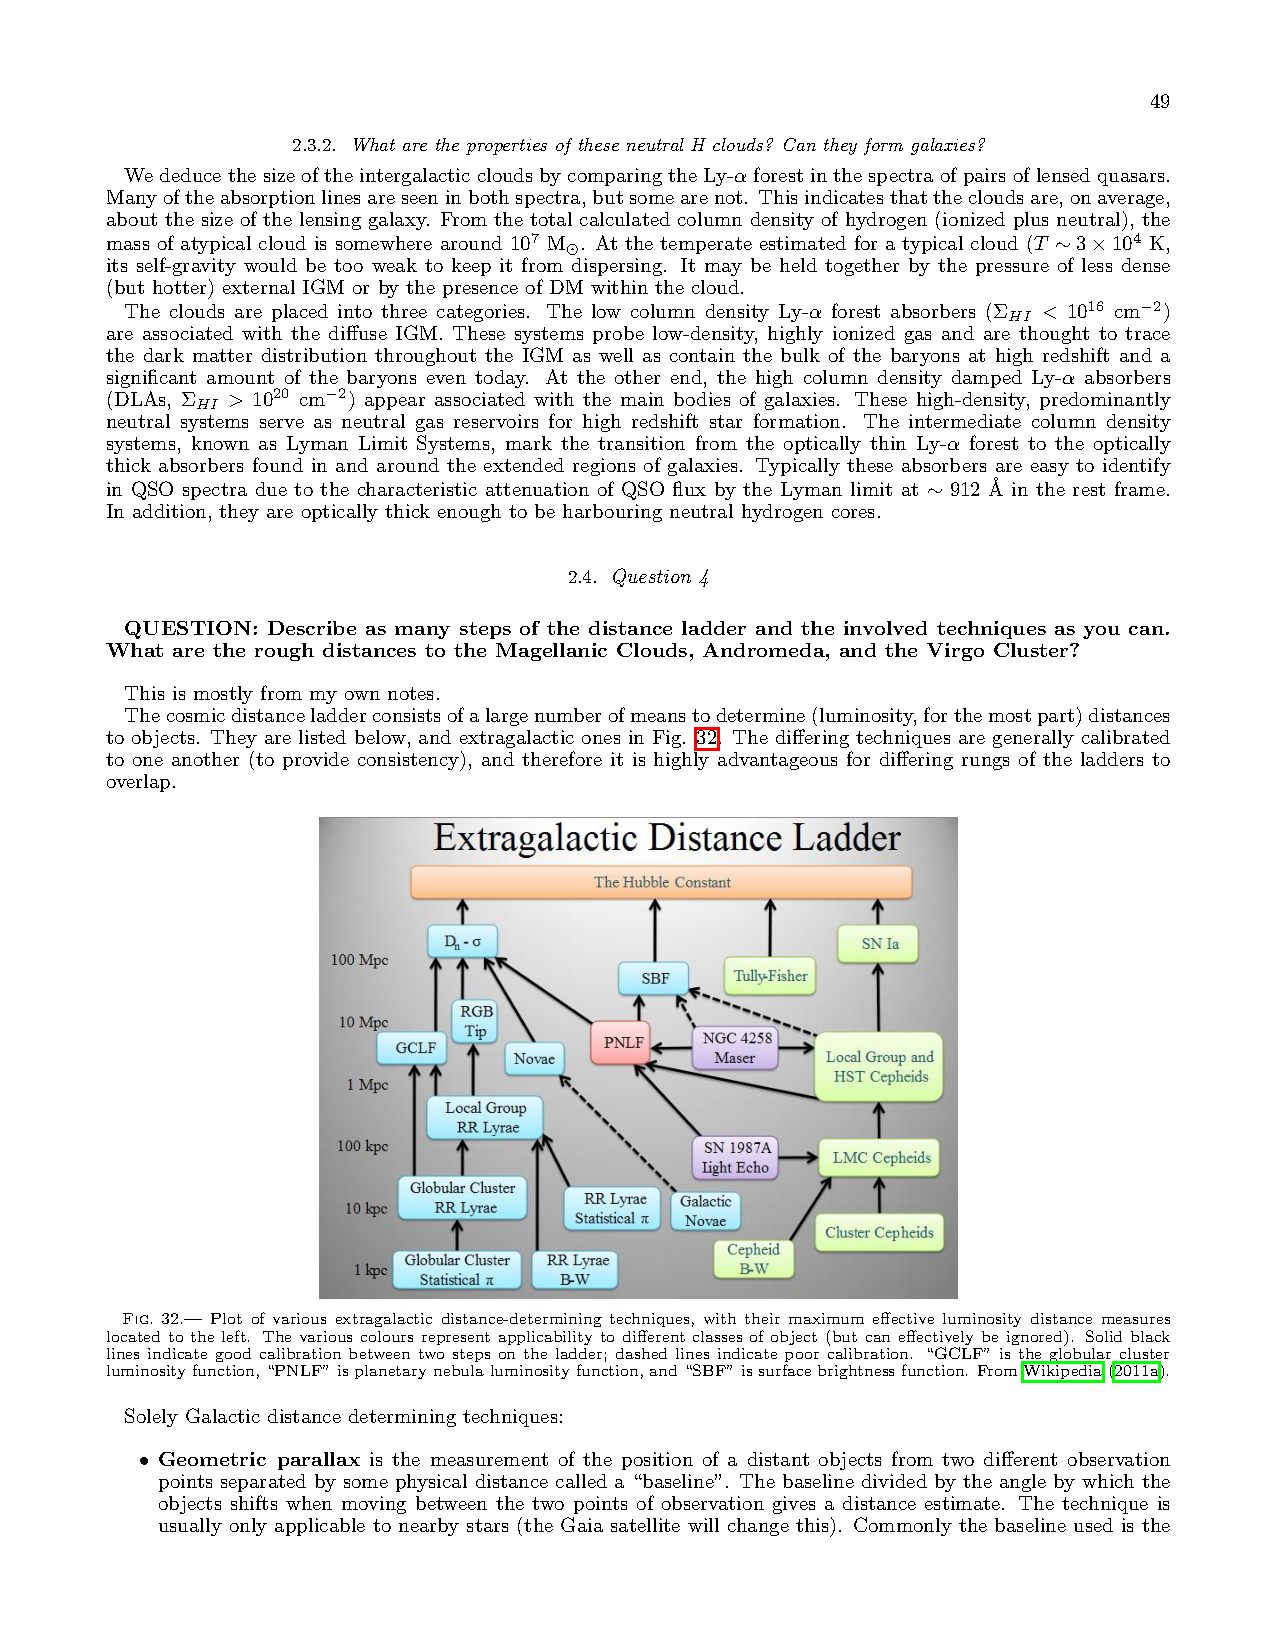
\includepdf[pagecommand=\subsection{Q7) Zhu ExtraGal Q4},pages=1]{cosmo_extragal/Zhu/Zhu_Q7}\includepdf[pages=2-]{cosmo_extragal/Zhu/Zhu_Q7}

% section q7_the_distance_ladder (end)


% -----------------------------------------------------------------------------
%                                      Q8
% -----------------------------------------------------------------------------

\section{Q8) Other Methods for Parameter Constraints} % (fold)
\label{sec:q8_other_methods_for_parameter_constraints}
\questiontext{Describe a method, other than Type Ia supernovae and CMB foregrounds, by which the cosmological parameters can be determined by astronomical observations, and describe the current status of constraints from this method.}


	% External Answers
	\includepdf[pagecommand=\subsection{Q8) Ludwig Cosmo Q7},pages=9]{cosmo_extragal/Ludwig/Cosmology}

	\includepdf[pagecommand=\subsection{Q8) Herman Cosmo Q8},scale=.93,offset=0 -14,pages=9]{cosmo_extragal/Herman/1_Cosmology}\includepdf[pagecommand=\large{Q8) Herman Cosmo Q8},scale=.93,offset=0 -14,pages=10]{cosmo_extragal/Herman/1_Cosmology}

	\includepdf[pagecommand=\subsection{Q8) Campbell Cosmo Q8},scale=.93,offset=0 -14,pages=40]{cosmo_extragal/Campbell/cosmology}\includepdf[pagecommand=\large{Q8) Campbell Cosmo Q8},scale=.93,offset=0 -14,pages=41-42]{cosmo_extragal/Campbell/cosmology}

% section q8_other_methods_for_parameter_constraints (end)


% -----------------------------------------------------------------------------
%                                      Q9
% -----------------------------------------------------------------------------

\section{Q9) CMB Polarization} % (fold)
\label{sec:q9_cmb_polarization}
\questiontext{Why is the cosmic microwave background expected to be weakly polarized, and what is practically required to observe this signal?}


	% External Answers
	\includepdf[pagecommand=\subsection{Q9) Ludwig Cosmo Q8},pages=10]{cosmo_extragal/Ludwig/Cosmology}

	\includepdf[pagecommand=\subsection{Q9) Herman Cosmo Q9},scale=.93,offset=0 -14,pages=11]{cosmo_extragal/Herman/1_Cosmology}

	\includepdf[pagecommand=\subsection{Q9) Campbell Cosmo Q9},scale=.93,offset=0 -14,pages=43]{cosmo_extragal/Campbell/cosmology}\includepdf[pagecommand=\large{Q9) Campbell Cosmo Q9},scale=.93,offset=0 -14,pages=44]{cosmo_extragal/Campbell/cosmology}

% section q9_cmb_polarization (end)


% -----------------------------------------------------------------------------
%                                      Q10
% -----------------------------------------------------------------------------

\section{Q10) CMB Secondary Anisotropies} % (fold)
\label{sec:q10_cmb_secondary_anisotropies}
\questiontext{Our view of the cosmic microwave background is affected by what is along the line of sight. Give two examples of CMB secondary anisotropies that also provide information about the cosmic parameters.}

	TSZ gives tau, amplifies Omega M

	ISW give H0 and Omega Lambda

	% External Answers
	\includepdf[pagecommand=\subsection{Q10) Ludwig Cosmo Q9},pages=11]{cosmo_extragal/Ludwig/Cosmology}

	\includepdf[pagecommand=\subsection{Q10) Herman Cosmo Q10},scale=.93,offset=0 -14,pages=12]{cosmo_extragal/Herman/1_Cosmology}

	\includepdf[pagecommand=\subsection{Q10) Campbell Cosmo Q10},scale=.93,offset=0 -14,pages=45]{cosmo_extragal/Campbell/cosmology}\includepdf[pagecommand=\large{Campbell Cosmo Q10},scale=.93,offset=0 -14,pages=46-49]{cosmo_extragal/Campbell/cosmology}

% section q10_cmb_secondary_anisotropies (end)


% -----------------------------------------------------------------------------
%                                      Q12
% -----------------------------------------------------------------------------

\section{Q11) Cosmological Inflation} % (fold)
\label{sec:q11_cosmological_inflation}
\questiontext{Describe cosmological inflation. List at least three important observations it is intended to explain.}


	% External Answers
	\includepdf[pagecommand=\subsection{Ludwig Cosmo Q10},pages=12]{cosmo_extragal/Ludwig/Cosmology}

	\includepdf[pagecommand=\subsection{Herman Cosmo Q11},scale=.93,offset=0 -14,pages=13]{cosmo_extragal/Herman/1_Cosmology}\includepdf[pagecommand=\large{Herman Cosmo Q11},scale=.93,offset=0 -14,pages=14]{cosmo_extragal/Herman/1_Cosmology}

% section q11_cosmological_inflation (end)


% -----------------------------------------------------------------------------
%                                      Q12
% -----------------------------------------------------------------------------

\section{Q12) Two-Point Correlation Function (2PCF)} % (fold)
\label{sec:q12_two_point_correlation_function}
\questiontext{Define the two-point correlation function of a Gaussian random field. How is it related to the power spectrum of that field? Describe how the above two concepts are used in cosmology.}

	\subsubsection{Short Summary} % (fold)
	\label{ssub:short_summary}

		The two point correlation function (2PCF) -- $\xi(R)$ -- describes the excess likelihood over a random distribution of finding 2 galaxies separated by a distance $R$. Equivalently, the 2PCF is the probability of finding a galaxy at some point $x$ given another galaxy $R$ away\footnote{this definition is useful for actually evaluating the 2PCF}.

		A Gaussian Random Field (field) is a stochastic process in spatial coordinates defined by at least one Gaussian kernel. The power spectrum describes the power per scale-length from each kernel.

		The initial conditions of the universe (QM fluctuations during Inflation) are thought to be a GRF with a scale-invariant spectrum. This means that the amplitudes are independent of the scale-length of the Gaussians. Now, the universe is not scale-independent -- The BAO ($\sim 150 \Mpc$) scale is the peak of galaxy clustering.

	% subsubsection short_summary (end)


	\subsubsection{Equations} % (fold)
	\label{ssub:equations}

		From empirical fits, the \textbf{2PCF} is given by

		\begin{equation*}\label{eq:q12_2pcf}
		    \xi_{g}(r) = \left(\frac{r}{r_0}\right)^{-\gamma} \ \ [{\rm dimensionless}],
		\end{equation*}

		{\noindent}where $r_0\sim5\,\inv{h}\, \Mpc$ is the correlation length and $\gamma\simeq1.7$ is the slope. This relation is reasonable over a range of separations: $0.2\inv{h} \Mpc \lessim r \lessim 30\inv{h} \Mpc$. The 2PCF is related to the \textbf{power spectrum} $P(k)$ via the Fourier transform,

		\begin{align*}\label{eq:q12_power_spectrum}
		    P(k) = 2\pi \int\limits_0^\infty \frac{\sin(kx)}{kx}\xi_{g}(x) x^2 \dif{x} \ \ [{\rm dimensionless}].
		\end{align*}
	
	% subsubsection equations (end)

	\subsubsection{Gaussian Random Field} % (fold)
	\label{ssub:gaussian_random_field}

		\begin{displayquote}
			``One way of constructing a GRF is by assuming that the field is the sum of a large number... of plane waves with uniformly distributed random phase... At any point, the sum of these individual plane-wave contributions will exhibit a Gaussian distribution. This type of GRF is completely described by its power spectral density.\\
			Suppose f(x) is the value of a GRF at a point x in some D-dimensional space. If we make a vector of the values of f at N points, x1, ..., xN, in the D-dimensional space, then the vector (f(x1), ..., f(xN)) will always be distributed as a multivariate Gaussian''\\
			(Modified from \href{https://en.wikipedia.org/wiki/Gaussian_random_field}{Wikipedia}).
		\end{displayquote}

	
	% subsubsection gaussian_random_field (end)

	% External Answers
	\includepdf[pagecommand=\subsection{Q12) Herman Cosmo Q13},scale=.93,offset=0 -14,pages=16]{cosmo_extragal/Herman/1_Cosmology}
	\includepdf[pagecommand=\subsection{Q12) Campbell Cosmo Q13},scale=.93,offset=0 -14,pages=56]{cosmo_extragal/Campbell/cosmology}\includepdf[pagecommand=\large{Q12) Campbell Cosmo Q13},scale=.93,offset=0 -14,pages=57-58]{cosmo_extragal/Campbell/cosmology}


% section q12_two_point_correlation_function (end)


% -----------------------------------------------------------------------------
%                                      Q13
% -----------------------------------------------------------------------------

\section{Q13) Angular Power Spectrum} % (fold)
\label{sec:q13_angular_power_spectrum}
\questiontext{How is the angular (Cl) power spectrum of the CMB related to the matter power spectrum and how can we use the Cls to learn about the initial conditions of the universe?}

    \subsection{Short Summary}
        The angular power spectrum of the CMB is \textit{sourced} by the density fluctuations that the matter power spectrum describes. That is, hot and cold spots in the CMB temperature arise from photons freely streaming out of over- and under-dense regions (respectively). The acoustic peaks in the CMB are so-named because they result from the Baryon Acoustic Oscillations (BAOs) in the matter-radiation plasma that existed prior to recombination.  

\subsection{Campbell} % (fold)
\label{sub:campbell}

{\noindent}\textbf{CMB angular power spectrum}: The comparison between the predicted acoustic peak scale and its angular extent provides a measurement of the angular diameter distance to recombination. The angular diameter distance in turn depends on the spatial curvature and expansion history of the Universe. Assuming the size of the Universe's horizon at the time of recombination and the distance to the last scattering surface, the geometry (or curvature) of the Universe can be measured using the angular size of the first peak of the angular power spectrum. If the first peak is at $\ell\sim220$, the Universe is flat, whereas if the first peak is at $\ell<220$ or $\ell>220$, the Universe is open or closed, respectively.

{\noindent}\textbf{BAOs}: The peaks in the CMB angular power spectrum are the result of compressions and expansions of the baryonic acoustic oscillations: the first and second peaks being the first compression and first decompression, respectively, etc. Given that the first compression happened on scales of the sound horizon at the time of last scattering, the first peak in the CMB angular power spectrum should tell you at what that scale was. This scale (i.e., the sound horizon) can be compared to what would be expected for a flat Universe -- if it is smaller, the Universe is open whereas if it is larger, the Universe is closed (if they're equal, the Universe is of course flat).

% subsection campbell (end)

% External Answers

% section q13_angular_power_spectrum (end)


% -----------------------------------------------------------------------------
%                                      Q14
% -----------------------------------------------------------------------------

\newpage
\section{Q14) Positive Cosmological Constant} % (fold)
\label{sec:q14_positive_cosmological_constant}
\questiontext{Consider a cosmological model including a positive cosmological constant. Show that, in such a model, the expansion factor eventually expands at an exponential rate. Sketch the time dependence of the expansion factor in the currently favoured cosmological model.
}

    \subsection{Short Summary}
        


	% External Answers
	\includepdf[pagecommand=\subsection{Q14) Ludwig Cosmo Q13},pages=15]{cosmo_extragal/Ludwig/Cosmology}

	\includepdf[pagecommand=\subsection{Q14) Herman Cosmo Q14},scale=.93,offset=0 -14,pages=17]{cosmo_extragal/Herman/1_Cosmology}

	\includepdf[pagecommand=\subsection{Q14) Campbell Cosmo Q14},scale=.93,offset=0 -14,pages=59]{cosmo_extragal/Campbell/cosmology}\includepdf[pagecommand=\large{Q14) Campbell Cosmo Q14},scale=.93,offset=0 -14,pages=60-61]{cosmo_extragal/Campbell/cosmology}

% section q14_positive_cosmological_constant (end)


% -----------------------------------------------------------------------------
%                                      Q15
% -----------------------------------------------------------------------------

\section{Q15) Epoch of Reionization} % (fold)
\label{sec:q15_epoch_of_reionization}
\questiontext{Define and describe the epoch of reionization. What are the observational constraints on it?}

    \subsection{Short Summary}
        The Universe was largely neutral after recombination. The earliest galaxies/quasars emit photo-ionizing radiation which ionizes all of the neutral gas around it. This results in the Gunn-Peterson trough. 


	% External Answers
	\includepdf[pagecommand=\subsection{Q15) Ludwig Cosmo Q14},pages=16]{cosmo_extragal/Ludwig/Cosmology}

	\includepdf[pagecommand=\subsection{Q15) Herman Cosmo Q15},scale=.93,offset=0 -14,pages=18]{cosmo_extragal/Herman/1_Cosmology}\includepdf[pagecommand=\large{Herman Cosmo Q15},scale=.93,offset=0 -14,pages=19]{cosmo_extragal/Herman/1_Cosmology}

	\includepdf[pagecommand=\subsection{Q15) Campbell Cosmo Q15},scale=.93,offset=0 -14,pages=62]{cosmo_extragal/Campbell/cosmology}\includepdf[pagecommand=\large{Q15) Campbell Cosmo Q15},scale=.93,offset=0 -14,pages=63-70]{cosmo_extragal/Campbell/cosmology}
    \subsection{Cosmology Class Fall 2019: Martine's Notes}
    Define and describe:
    \par
    Today, the IGM is mainly ionized. The ISM is mostly ionized.
    Two main constraints on reionization: CMB spectrum and the spectra of quasars.
    \par
    \textbf{Spectra of quasars}
    \par
    If you can find quasars with the Gunn-Peterson trough, then you know there was a period of time where the universe was neutral.
    What this would look like: Lyman alpha peak, then at redder frequencies an extended trough, then the Lyman-alpha forest at redder frequencies from clumps of neutral hydrogen.
    
    From this evidence, reionization happens at $z\approx6$. Galaxies at higher redshifts have been seen with this trough.
    \par
    \textbf{CMB evidence}
    \par
    CMB scatters off of ionized universe. Different electrons which scatter CMB photons see different quadropoles and thus the scattered light is polarized. The variations in the polarization are largest at large scales because far-apart electrons see the most different version of the CMB. Nearby electrons see similar CMB quadropole. There is a peak at low $\ell$ in the $(\ell)(\ell+1)C_{ell}^{EE}$ power spectrum. This will be higher in power if reionization happened earlier, because the universe was denser at that point so there was more scattering and thus more polarization. It will also be at lower ${ell}$ if reionization happened earlier, because the distance between an electron which sees one CMB quadropole and another electron which sees an entirely different CMB quadropole is smaller at earlier times (I think; don't quote me on that last bit).
% section q15_epoch_of_reionization (end)


% -----------------------------------------------------------------------------
%                                      Q16
% -----------------------------------------------------------------------------

\section{Q16) 21 CM Hydrogen} % (fold)
\label{sec:q16_21_cm_hydrogen}
\questiontext{The 21 cm line of hydrogen is expected to show up in absorption against the cosmic microwave background at some redshifts, and in emission at other redshifts. What physical processes lead to this behaviour?}

	\subsection{Short Summary} % (fold)
	\label{sub:subsection_name}
	
	% subsection subsection_name (end)


	% External Answers
	\includepdf[pagecommand=\subsection{Q16) Ludwig Cosmo Q15},pages=17]{cosmo_extragal/Ludwig/Cosmology}

	\includepdf[pagecommand=\subsection{Q16) Herman Cosmo Q16},scale=.93,offset=0 -14,pages=20]{cosmo_extragal/Herman/1_Cosmology}

	\includepdf[pagecommand=\subsection{Q16) Campbell Cosmo Q16},scale=.93,offset=0 -14,pages=71]{cosmo_extragal/Campbell/cosmology}\includepdf[pagecommand=\large{Q16) Campbell Cosmo Q16},scale=.93,offset=0 -14,pages=72-74]{cosmo_extragal/Campbell/cosmology}

% section q16_21_cm_hydrogen (end)


% -----------------------------------------------------------------------------
%                                      Q17
% -----------------------------------------------------------------------------

\section{Q17) Cosmic Neutrino Background} % (fold)
\label{sec:q17_cosmic_neutrino_background}
\questiontext{What are the similarities and differences between the cosmic neutrino background and the cosmic microwave background?}


	% External Answers
	\includepdf[pagecommand=\subsection{Q17) Ludwig Cosmo Q17},pages=19]{cosmo_extragal/Ludwig/Cosmology}

	\includepdf[pagecommand=\subsection{Q17) Herman Cosmo Q18},scale=.93, offset=0 -14,pages=22]{cosmo_extragal/Herman/1_Cosmology}

	\includepdf[pagecommand=\subsection{Q17) Campbell Cosmo Q18},scale=.93,offset=0 -14,pages=82]{cosmo_extragal/Campbell/cosmology}\includepdf[pagecommand=\large{Q17) Campbell Cosmo Q18},scale=.93,offset=0 -14,pages=83]{cosmo_extragal/Campbell/cosmology}

    \subsection{Cosmology Class Fall 2019: Martine's Notes}
    
    \par
    \begin{equation}
        a + b \leftrightarrow c + d
    \end{equation}
    
    \begin{equation}
        f = \frac{1}{e^{E-\mu}/kT \pm 1}
    \end{equation}
    Early universe, at very high temperatures, every particle has equal likelihood. $\mu$ is 1 when T is high.
    
    At $kT>511$keV:
    \begin{equation}\label{neutrino_int}
        \nu_e + \bar{\nu_e} \leftrightarrow e^+ + e^-
    \end{equation}
    
    Define the interaction rate, $\Gamma$. Define the expansion rate, $H$. When $\Gamma >> H$, lots of interactions. When $\Gamma \leq H$, you get freeze out.
    
    Let's talk about
    
    \begin{equation}
        p^+ + e^- \leftrightarrow n + \nu_e
    \end{equation}
    \begin{equation}
        \frac{n_n}{n_p} = e^{-Q/T}
    \end{equation}
    \begin{equation}
        Q = \Delta M = 1.3 MeV
    \end{equation}
    (Q is the difference in the masses of the two particles.)
    
    At around T$\approx$1 MeV, or around 1 second, the interaction rate of Equation \ref{neutrino_int} goes below $H$ and the numbers of neutrinos freezes out.
    
    The temperature of the C$\nu$B is $T_{\nu} = 1.95K \approx 0.17 meV$.
    
    Around the same time, another process stops:
    \begin{equation}
        e^+ +  e^- \leftrightarrow \gamma + \gamma
    \end{equation}
    The likelihood of this reaction (cross section) is higher than of \ref{neutrino_int}. But then after $T < 511$ keV, the gammas can no longer interact to form electrons because they don't have enough energy. But the electron-positron interaction keeps going. 
    
    Cosmic neutrino background decoupled earlier, and didn't get the extra energy from electron-positron annihilation added to it. But the CMB did.
    
    Neutrinos have mass. The C$\nu$B contributes to the mass density of the universe.
    \begin{equation}
        \Omega_\nu h^2 = \Sigma_i \frac{M_{\nu,i}}{94 eV}
    \end{equation}
    We know:
    $\Sigma_i M_{\nu,i} > 60$ meV: Neutrino oscillation experiments. 
    $\Sigma_i M_{\nu,i} < 120$ meV: Fits to the CMB.
    \textbf{Barth's follow up question}
    \par
    What makes detection of the Cosmic Neutrino background challenging? If it could be measured at the same resolution and precision as the cosmic microwave background, what would it’s angular power spectrum look like?
% section q17_cosmic_neutrino_background (end)


% -----------------------------------------------------------------------------
%                                      Q18
% -----------------------------------------------------------------------------

\newpage
\section{Q18) Dark Matter Candidates} % (fold)
\label{sec:q18_dark_matter_candidates}
\questiontext{Give three examples of possible dark matter candidates (current or historical). What is their status observationally?}


	% External Answers
	\includepdf[pagecommand=\subsection{Herman Cosmo Q20},scale=.93, offset=0 -14,pages=24]{cosmo_extragal/Herman/1_Cosmology}\includepdf[pages=25]{cosmo_extragal/Herman/1_Cosmology}

	\includepdf[pagecommand=\subsection{Q18) Campbell Cosmo Q20},scale=.93,offset=0 -14,pages=85]{cosmo_extragal/Campbell/cosmology}

% section q18_dark_matter_candidates (end)


% -----------------------------------------------------------------------------
%                                      Q19
% -----------------------------------------------------------------------------

\section{Q19) Galaxy Clusters} % (fold)
\label{sec:q19_galaxy_clusters}
\questiontext{What are galaxy clusters? List and explain three methods for detecting them or determining their basic properties.}


	% External Answers
	\includepdf[pagecommand=\subsection{Herman ExtraGal Q13},scale=.93, offset=0 -14,pages=14]{cosmo_extragal/Herman/2_Extragalactic}\includepdf[pagecommand=\large{Herman ExtraGal Q13},scale=.93, offset=0 -14,pages=15]{cosmo_extragal/Herman/2_Extragalactic}

% section q19_galaxy_clusters (end)


% -----------------------------------------------------------------------------
%                                      Q20
% -----------------------------------------------------------------------------


\section{Star Formation Quenching} % (fold)
\label{sec:star_formation_quenching}
\questiontext{What is star formation quenching in galaxies? What is the evidence for it, and why is it thought to happen?}


	% External Answers
	\includepdf[pagecommand=\subsection{Herman ExtraGal Q14},scale=.93, offset=0 -14,pages=16]{cosmo_extragal/Herman/2_Extragalactic}\includepdf[pagecommand=\large{Herman ExtraGal Q14},scale=.93, offset=0 -14,pages=17]{cosmo_extragal/Herman/2_Extragalactic}

% section star_formation_quenching (end)


% -----------------------------------------------------------------------------
%                                      OLD
% -----------------------------------------------------------------------------

\section{OLD COSMOLOGY QUESTIONS, NOT IN THIS QUAL} % (fold)
\label{sec:old_cosmology_questions_not_in_this_qual}

	\includepdf[pagecommand=\subsection{Herman Cosmo Q5},scale=.93, offset=0 -14,pages=6]{cosmo_extragal/Herman/1_Cosmology}

	\includepdf[pagecommand=\subsection{Herman Cosmo Q12},scale=.93, offset=0 -14,pages=15]{cosmo_extragal/Herman/1_Cosmology}

	\includepdf[pagecommand=\subsection{Herman Cosmo Q17},scale=.93, offset=0 -14,pages=21]{cosmo_extragal/Herman/1_Cosmology}

	\includepdf[pagecommand=\subsection{Herman Cosmo Q19},scale=.93, offset=0 -14,pages=23]{cosmo_extragal/Herman/1_Cosmology}


% -----------------------------------------------------------------------------
%                                      Q3
% -----------------------------------------------------------------------------

\subsection{OLD Q3) CDM Spectrum evolution} % (fold)
\label{sub:old_q3_cdm_spectrum_evolution}
\questiontext{Outline the development of the Cold Dark Matter spectrum of density fluctuations from the early universe to the current epoch.}


	% External Answers
	\includepdf[pagecommand=\subsubsection{Q3) Ludwig Cosmo Q3},pages=5]{cosmo_extragal/Ludwig/Cosmology}

	\includepdf[pagecommand=\subsubsection{Q3) Herman Cosmo Q3},scale=.93,offset=0 -14,pages=3]{cosmo_extragal/Herman/1_Cosmology}\includepdf[pagecommand=\large{Herman Cosmo Q3},scale=.93,offset=0 -14,pages=4]{cosmo_extragal/Herman/1_Cosmology}
	\includepdf[pagecommand=\subsubsection{Q3) Campbell Cosmo Q3},scale=.93,offset=0 -14,pages=11]{cosmo_extragal/Campbell/cosmology}\includepdf[pagecommand=\large{Q3) Campbell Cosmo Q3},scale=.93,offset=0 -14,pages=12-20]{cosmo_extragal/Campbell/cosmology}

	\includepdf[pagecommand=\subsubsection{Q3) Zhu Cosmo Q3},pages=1]{cosmo_extragal/Zhu/Zhu_Q3}\includepdf[pages=2-]{cosmo_extragal/Zhu/Zhu_Q3}

% subsection old_q3_cdm_spectrum_evolution (end)

% section old_cosmology_questions_not_in_this_qual (end)

\end{document}

%%%%%%%%%%%%%%%%%%%%%%%%%%%%%%%%%%%%%%%%%%%%%%%%%%%%%%%%%%%%%%%%%%%%%%%%%%%%%%#